\documentclass[12pt,a4paper]{article}

\usepackage[UTF8]{ctex}
\usepackage[scale=0.8]{geometry}
\usepackage{latexsym,amsmath,amsfonts,amssymb,mathrsfs,bm}
\usepackage{abstract,appendix,titlesec,titletoc}
\usepackage{diagbox,booktabs,longtable,tabularx}
\usepackage[amsmath,thmmarks,hyperref]{ntheorem}
\usepackage{fancyhdr,indentfirst}
\usepackage[colorlinks=ture]{hyperref}
\usepackage{makeidx,cleveref}
\usepackage[sort&compress, numbers]{natbib}
\usepackage{graphicx,epsfig,subfig}
\usepackage{algorithm,algorithmicx,algpseudocode}
\usepackage{xcolor}

%\setlength{\lineskip}{\baselineskip}
\setlength{\parskip}{0.5\baselineskip}

\theoremstyle{plain}
\newtheorem{definition}{定义}
\newtheorem{example}{例}
\newtheorem{theorem}{定理}
\newtheorem{lemma}{引理}
\newtheorem{corollary}{推论}
\newtheorem{remark}{注}
\newtheorem{proposition}{性质}

\newcommand{\diag}{\mathrm{diag}}
\newcommand{\tr}{\mathrm{tr}}
\newcommand{\Rnum}{\mathbb{R}}
\newcommand{\Cnum}{\mathbb{C}}
\newcommand{\Znum}{\mathbb{Z}}
\newcommand{\Nnum}{\mathbb{N}}
\newcommand{\bx}{\mathbf{x}}
\newcommand{\by}{\mathbf{y}}
\newcommand{\bn}{\mathbf{n}}

\title{一种基于最小二乘和流连续性的有限体积格式}
\author{sis-flag}
\date{\today}

\begin{document}

\maketitle

\section*{问题介绍}

区域$\Omega$是二维多边形区域。我们要在区域上求解稳态扩散问题
\begin{equation}
\begin{split}
- \nabla \cdot (a \, \nabla u)= f & \quad x \in \Omega \\
u = u_0 & \quad x \in \partial \Omega
\end{split}
\end{equation}
其中$u(x)$是未知函数,$a(x)$是$2 \times 2$对称正定的矩阵,表示张量型的扩散系数。

\section*{有限体积格式}

我们希望在扭曲的多边形网格上求解方程。网格中的多边形叫做控制体。这里我们要求控制体至少是星形的,控制体的中心到其中任何一点的连线还在控制体中。

在控制体$K$上对方程两边积分,用散度定理得到
\begin{align*}
- \int_{K} \nabla \cdot (\kappa(x) \, \nabla u(x)) \ dx = - \sum_{e \in \mathcal{E}(K)} \int_{e} (\kappa(x) \, \nabla u(x)) \cdot n_{K, e} \ dx = \int_{K} f(x) \ dx
\end{align*}
其中$n_{K, e}$是控制体在边界上的外法方向,$e = AB$是控制体的边。

我们用函数在单元中心处的值代替边界上的值,也就是假设扩散系数和未知函数的梯度在每个单元上近似为常数。$\kappa(x) \, \nabla u(x) = \kappa(K) \, \nabla u(K) + \mathcal{O}(h)$。得到
\begin{align*}
F_{K, e} = - \int_{e} (\kappa(K) \, \nabla u(K)) \cdot n_{K, e} \ dx + \mathcal{O}(h^2)
\end{align*}
这里$K$有时表示控制体,有时表示控制体中心坐标。

\begin{figure}[h]
\centering
\caption{数值格式的模板}
\label{f1}
\end{figure}

如图\ref{f1},边$e = AB$是一条位于内部的边,它的中点为$E$,方向向量为$t_e$,法向为$n_e$,$n_e$从单元$K$指向单元$L$。在图中红色的四边形中,我们定义近似解$\hat{u}(x)$,它在三角形$KAB$和$LAB$上是线性函数。
\begin{equation*}
\hat{u}(x) = \left\{
\begin{split}
g_K^T \, x + c_K \quad x \in K \\
g_L^T \, x + c_L \quad x \in L
\end{split}
\right.
\end{equation*}

已知方程的解$u(x)$是连续的,而且流量$a(x) \, \nabla u(x)$也连续。为了使两个单元上计算出的流量相同,需要满足
\begin{align*}
g_K^T \, a(K) \, n_e = g_L^T \, a(L) \, n_e = F_e \qquad
g_K^T \, t_e = g_L^T \, t_e \qquad
g_K^T \, x_E + c_K = g_L^T \, x_E + c_L \qquad
\end{align*}
此时边界上的流量就是$|e| F_e$。

此外,我们希望$\hat{u}(x)$尽可能贴近解,也就是
\begin{align*}
\min \; \sum_{\alpha = K,L,A,B} |u(\alpha) - \hat{u}(\alpha)|^2
\end{align*}

这个鬼东西的解写不出来显式表达式,就尴尬了。。。

%\subsection{九点格式}
%
%把联合法向量分解成$\overrightarrow{KA}, \overrightarrow{KB}$的组合,即
%\begin{align*}
%\kappa(K)^T n_{K, e} = \alpha_A \, \overrightarrow{KA} + \alpha_B \, \overrightarrow{KB}
%\end{align*}
%根据方向导数的性质
%\begin{align*}
%\nabla u(K) \cdot \overrightarrow{KA} = u(A) - u(K) + \mathcal{O}(h)
%\end{align*}
%得到流量表示为
%\begin{align*}
%F_{K, e} = |e| \; (\alpha_A \, (u(K) - u(A)) + \alpha_B \, (u(K) - u(B))) + \mathcal{O}(h^2)
%\end{align*}
%
%网格节点处的函数值可以通过相邻的网格中心处函数值线性插值得到。假设我们已经找到了一种二阶插值
%\begin{align*}
%u(A) = \sum_{K \in \mathcal{N}(A)} w_{K,A} u(K) + \mathcal{O}(h^2)
%\end{align*}
%此时就可以把边界上的流量用单元中心表示出来。对于边$AB$上的流量,需要用到与$A$和$B$相邻的所有单元。
%
%同理,在相邻的另一个单元上,我们也可以得到另一侧的流量$F_{L, e}$。既然两个流量都是二阶的,考虑到流守恒的要求,我们可以把两个流平均起来,就得到了最终的流量。(此处要注意符号,$K$和$L$上计算的流量都是以向外为正方向)
%\begin{align*}
%\mathcal{F}_{K, e} = \frac12 (F_{K, e} - F_{L, e})
%\end{align*}
%
%此时计算某个单元的流量,需要用到和它共顶点的所有单元。在四边形网格中,与某个单元共顶点的单元有九个,因此这个格式被叫做九点格式。
%
%九点格式具有二阶精度,但不能保正。
%
%\subsection{五点格式}
%
%在控制体的顶点中选择$P_1, P_2$,使联合法向量可以表示成这两个向量的凸组合
%\begin{align*}
%\kappa(K)^T n_{K, e} = \alpha_1 \, \overrightarrow{K P_1} + \alpha_2 \, \overrightarrow{k P_2}
%\end{align*}
%根据方向导数的性质
%\begin{align*}
%\nabla u(K) \cdot \overrightarrow{K P_1} = u(P_1) - u(K) + \mathcal{O}(h)
%\end{align*}
%得到流量表示为
%\begin{align*}
%F_{K, e} = |e| \; (\alpha_1 \, (u(K) - u(P_1)) + \alpha_2 \, (u(K) - u(P_2))) + \mathcal{O}(h^2)
%\end{align*}
%此时$\alpha_1,\alpha_2 > 0$。网格节点处的函数值同样通过相邻的网格中心处函数值线性插值得到。
%
%同理,在相邻的另一个单元上,我们也可以得到另一侧的流量$F_{L, e}$,对应凸组合的两个点是$P_3, P_4$。既然两个流量都是二阶的,考虑到流守恒的要求,我们可以把两个流加权平均起来,得到最终的流量。
%\begin{align*}
%\mathcal{F}_{K, e} = & \mu_K \, F_{K, e} - \mu_L \, F_{L, e} \\
%= & |e| \left(\mu_K \, (\alpha_1 + \alpha_2) \, u(K) - \mu_L \, (\alpha_3 + \alpha_4) \, u(L) \right) \\
%& - |e| \left(\mu_K \, (\alpha_1 \, u(P_1) + \alpha_2 \, u(P_2)) - \mu_L \, (\alpha_3 \, u(P_3) + \alpha_4 \, u(P_4)) \right)
%\end{align*}
%其中$\mu_K, \mu_L$是权重。
%
%这里我们要适当调整权重,让最终的线性方程组里面不出现节点函数值,也就是权重要满足
%\begin{align*}
%\left\{
%\begin{array}{l}
%\mu_K + \mu_L = 1 \\
%t_K \, \mu_K - t_L \, \mu_L = 0
%\end{array}
%\right.
%\end{align*}
%其中
%\begin{align*}
%t_K = \alpha_1 \, u(P_1) + \alpha_2 \, u(P_2), \quad t_L = \alpha_3 \, u(P_3) + \alpha_4 \, u(P_4)
%\end{align*}
%解出来得到
%\begin{align*}
%\mu_K = \frac{t_L}{t_K + t_L}, \quad \mu_L = \frac{t_K}{t_K + t_L}, \quad (t_K + t_L \neq 0). \qquad \mu_K = \mu_L = \frac12, \quad (t_K + t_L = 0).
%\end{align*}
%通过这样选取权重,可以在最终的线性方程组中只出现单元中心的值。因此这个格式被称作五点格式。
%
%如果有二阶保正插值,五点格式就是一个保正,二阶的数值格式,但注意到系数$t_K,t_L$和解有关,因此它是非线性的,要通过迭代法求解。
%
%\subsection{Picard迭代}
%
%注意到在数值格式中,$\mu_1,\mu_2$和节点处的函数有关,代入插值可以看出,方程组内$u(K)$的系数中仍然含有$u(K)$,因此这是一个非线性格式。
%
%求解五点格式,我们通常使用Picard迭代。具体步骤如下:
%\begin{enumerate}
%\item 选定初始值$u^{(0)}$。
%\item 计算线性插值,得到解$u^{(k)}$在节点上的值。
%\item 通过解在节点上的值,计算权重,装配矩阵$A(u^{(k)})$。
%\item 求解线性方程$A(u^{(k)}) \, u^{(k+1)} = F$,得到新的解$u^{(k+1)}$在单元中心处的值。
%\item 重复以上步骤,直到精度达标。
%\end{enumerate}
%
%对于五点格式,Picard迭代的收敛性目前还没有证明,不过它是目前最常用的非线性迭代方法。
%
%\section{插值方法}
%
%\subsection{保正条件}
%
%这里被插值的节点记为$A$,周围单元中心记为$K_1, K_2, \cdots$。
%
%在五点格式中,如果我们已经确保插值过程中,插值的系数全部为正数
%\begin{align*}
%u(A) \approx \sum w_{i} u(K_i), \quad w_{i} \geq 0
%\end{align*}
%此时,对于正的单元中心值$u(K_i) \geq 0$,得到的节点值也是正的。由于在格式中,联合法向量被表示成凸组合,因此得到$\alpha_1, \alpha_2, t_1, t_2, \mu_1, \mu_2 \geq 0$。因此对于非负的解,装配出的矩阵的转置就是M矩阵。
%
%\begin{lemma}
%M矩阵的性质。保正
%\end{lemma}
%\textbf{有时间仔细研究一下M矩阵的性质}
%
%\subsection{连续情况下的二阶条件}
%
%如果在节点附近,$u(x)$一阶导数连续,我们可以把函数在节点处Talyor展开
%\begin{align*}
%u(K_i) = u(A) + \frac{\partial u}{\partial x}(A) \, (x_i - x_A) + \frac{\partial u}{\partial y}(A) \, (y_i - y_A) + \mathcal{O}(h^2)
%\end{align*}
%在最终的插值中,我们希望消掉所有的一阶项,而且要满足权重相加为1。可以得到权重要满足的方程为
%\begin{align*}
%\left\{\begin{array}{l}
%w_1 + w_2 + \cdots w_n = 1 \\
%(x_1 - x_A) \, w_1 + (x_2 - x_A) \, w_2 + \cdots (x_n - x_A) \, w_n = 0 \\
%(y_1 - y_A) \, w_1 + (y_2 - y_A) \, w_2 + \cdots (y_n - y_A) \, w_n = 0 \\
%\end{array}\right.
%\end{align*}
%求保正插值,就相当于找上面的线性方程各分量都非负的解。
%
%\subsection{对偶网格插值}
%
%\begin{theorem}
%如果$A$点在$K_i$点组成的凸包(就是以这些点为顶点的凸多边形)里,以上方程一定有解,也就是一定存在保正插值。如果不在,则以上方程一定没有解。
%\end{theorem}
%\textbf{整个定理是我想出来的,证明后面补上。}
%
%这个定理说明对于网格很差的情况,用相邻单元中心对节点插值一定\textbf{不能}保正。我们需要想其它办法。
%
%以原网格的中心为节点,把和同一节点相邻的共边单元的中心之间连上边,这些边可以围成新的控制体。这样得到的网格叫做对偶网格。在边界处,我们要把边界上边的中点也补充到对偶网格的节点中去。这样,定理就可以表示为:如果节点在对偶网格对应的单元凸包内部,就可以保正插值,否则就不行。
%
%\begin{figure}[h]
%\centering
%%\includegraphics[width=0.4\linewidth]{dual}
%%\includegraphics[width=0.4\linewidth]{interp}
%\caption{对偶网格}
%\label{f2}
%\end{figure}
%
%注意到,原网格的节点$A$在对偶网格中,不一定在单元$K_1 K_2 \cdots$的内部,但是由于对偶网格铺满整个空间,因此节点一定在对偶网格的某个单元$L$的内部。我们只要在单元$L$内对节点进行插值,就一定是二阶保正的。
%
%如果有多于三个单元对节点进行插值,此时我们就有多于三个变量,但是线性约束只有三个,因此我们还有额外的自由度需要确定。在这里我们让权重在满足二阶和保正条件的同时,尽可能“平均”,也就是让它的方差$\mathrm{Var}(w) = \|w - w_0\|^2$最小。
%
%因此权重的确定转化为优化问题
%\begin{align}\label{p1}
%\min & \; \|w - w_0\|^2 \\
%s.t. & \; A w = b \quad w \geq 0
%\end{align}
%其中
%\begin{align*}
%A = \left(\begin{array}{cccc}
%1 & 1 & \cdots & 1 \\
%x_1 - x_A & x_2 - x_A & \cdots & x_n - x_A \\
%y_1 - y_A & y_2 - y_A & \cdots & y_n - y_A \\
%\end{array}\right)
%\quad
%b = \left(\begin{array}{c}
%1 \\
%0 \\
%0 \\
%\end{array}\right)
%\quad
%w_0 = \left(\begin{array}{c}
%1/n \\
%\vdots \\
%1/n \\
%\end{array}\right)
%\end{align*}
%
%我们直接把$w \geq 0$的约束拿掉,变成
%\begin{align}\label{p2}
%\min & \; \frac12 \|w - w_0\|^2 \\
%s.t. & \; A w = b
%\end{align}
%可以用拉格朗日乘数法得到优化问题的解。拉格朗日函数为
%\begin{align*}
%L(w, \lambda) = \frac12 (w - w_0)^T (w - w_0) + (A w - b)^T \lambda
%\end{align*}
%最优值条件为
%\begin{align*}
%\frac{\partial L}{\partial w} = w - w_0 + A^T \lambda = 0 \qquad A w = b
%\end{align*}
%解出来得到
%\begin{align*}
%\lambda = (A \, A^T)^{-1} (A \, w_0 - b) \qquad w = w_0 - A^T \lambda
%\end{align*}
%
%\begin{theorem}
%如果松弛后的问题\ref{p2}解全是正的,那它就是原问题\ref{p1}的解。如果松弛后的问题\ref{p2}解不满足$w \geq 0$,则原问题\ref{p1}无解。换言之,它们之间是充分必要条件。
%\end{theorem}
%目前没想到证明,但是我很确信这个定理是对的。
%
%\subsection{间断线附近的的二阶条件}
%
%上面说了$u(x)$二阶可导的情况,但是实际上方程的解不一定满足这样的要求,在扩散系数有间断的时候,在间断处并不能得到$\nabla u$可导,只能保证流连续性,也就是$\kappa \nabla u$可导。我们事先知道扩散系数在何处间断,因此可以把网格线放在间断线处,因此我们可以假设解在单元内部是二阶可导的。\cite{Sheng2008}
%
%\begin{figure}[h]
%\centering
%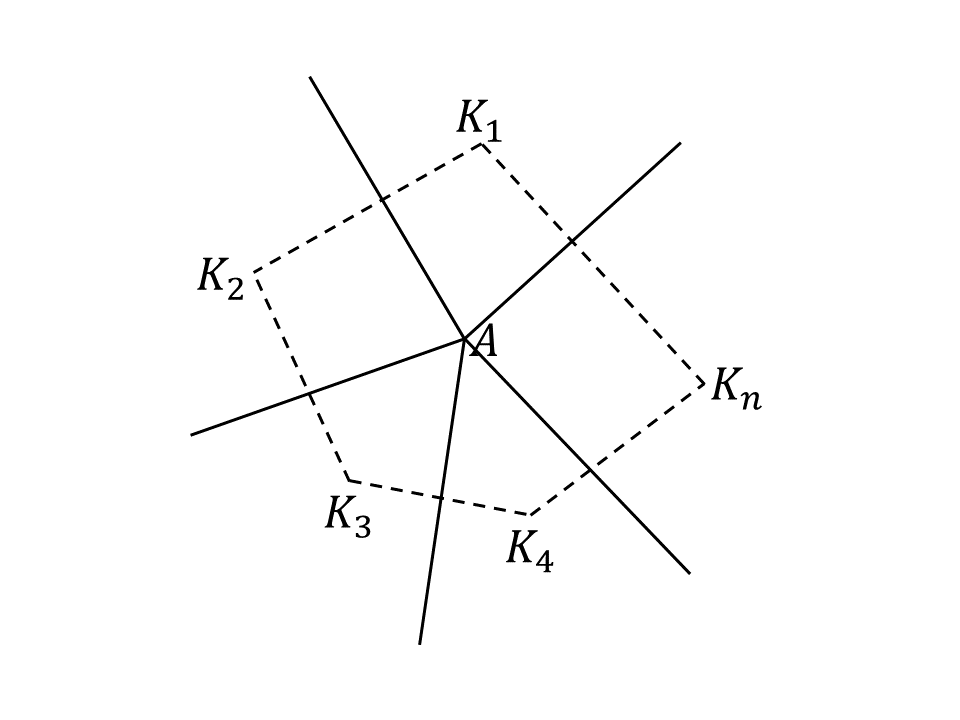
\includegraphics[width=0.3\linewidth]{stencil/interp1}
%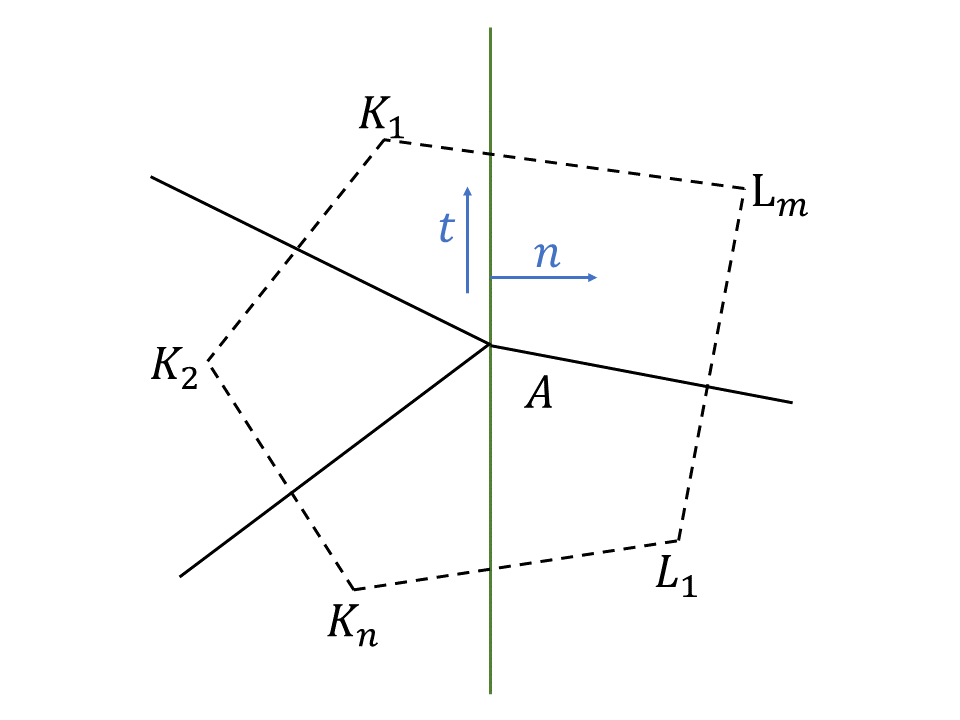
\includegraphics[width=0.3\linewidth]{stencil/interp2}
%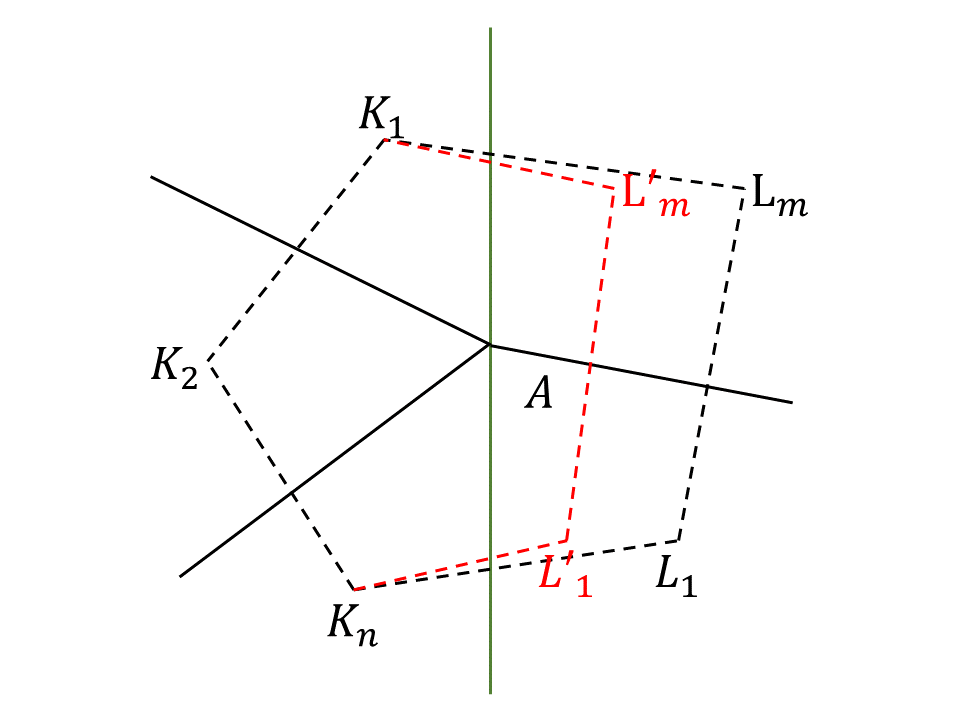
\includegraphics[width=0.3\linewidth]{stencil/interp3}
%\caption{插值模板}
%\label{f3}
%\end{figure}
%
%首先考虑简单的情况,假设扩散系数间断线是一条直线,节点$A$位于直线上。由于插值具有平移和旋转不变性,不失一般性,我们可以假设间断线和y轴平行。根据前面的分析,导数在左右两端不连续,设左边的单元是$K_1, K_2, \cdots, K_n$,右边的单元是$L_1, L_2, \cdots L_m$。两侧的扩散系数在$A$点的取值为$\kappa^{(K)}(A)$和$\kappa^{(L)}(A)$,两侧的导数分别为$\nabla u^{(K)}(A)$和$\nabla u^{(L)}(A)$。
%
%同样把每个单元上的解在节点处Taylor展开,对于左边的单元,单元中心处函数值近似为
%\begin{align*}
%u(K_i) = u(A) + \frac{\partial u}{\partial x}^{(K)}(A) \, (x_i - x_A) + \frac{\partial u}{\partial y}^{(K)}(A) \, (y_i - y_A) + \mathcal{O}(h^2)
%\end{align*}
%对于右边的单元,同理有
%\begin{align*}
%u(L_i) = u(A) + \frac{\partial u}{\partial x}^{(L)}(A) \, (x_i - x_A) + \frac{\partial u}{\partial y}^{(L)}(A) \, (y_i - y_A) + \mathcal{O}(h^2)
%\end{align*}
%注意这里的$K$和$L$单元不一定和$A$相邻,它们只是要去对节点进行插值的单元。
%
%设间断线对应的方向向量为$t_i = (0,1)^T$,法向量为$n_i = (1,0)^T$。因此两个单元之间的流连续条件为
%\begin{align*}
%n^T \, (\kappa^{(K)} \, \nabla u^{(K)}) = n^T \, (\kappa^{(L)} \, \nabla u^{(L)})
%\end{align*}
%由于解是连续的,解的梯度应该在切向相同
%\begin{align*}
%t_i^T \, \nabla u^{(K)} = t_i^T \, \nabla u^{(L)}
%\end{align*}
%通过梯度转移条件,可以看出在$y$方向两边的导数是一样的,即$\frac{\partial u}{\partial y}^{(L)} = \frac{\partial u}{\partial y}^{(K)} = \frac{\partial u}{\partial y}$。
%
%这里的矩阵
%\begin{align*}
%\left(\begin{array}{c}
%n^T \, \kappa^{(K)} \\
%t^T
%\end{array}
%\right)^{-1}
%\left(\begin{array}{c}
%n^T \, \kappa^{(L)} \\
%t^T
%\end{array}
%\right)
%\end{align*}
%叫做梯度转移矩阵,一边的梯度乘以这个矩阵就变成了另一边的梯度。
%
%得到的二阶保正性条件和前面类似,只是把矩阵改成
%\begin{align*}
%A = \left(\begin{array}{cccccc}
%1 & \cdots & 1 & 1 & \cdots & 1 \\
%x_1 - x_A & \cdots & x_n - x_A & d \, (x_{n+1} - x_A) & \cdots & d \, (x_{n+m} - x_A) \\
%y_1 - y_A & \cdots & y_n - y_A & y_{n+1} - y_A & \cdots & y_{n+m} - y_A
%\end{array}
%\right)
%\end{align*}
%其中$d = \frac{\partial u}{\partial x}^{(L)} / \frac{\partial u}{\partial x}^{(K)}$。
%
%如图,间断系数附近的插值就相当于在新的虚拟节点上进行插值。在左边,新的虚拟节点和原来相同,在右边,新的虚拟节点纵坐标和原来相同,横坐标会伸缩$d$倍。如果节点在新的虚拟节点组成的凸包里,就有二阶保正插值。
%
%如果$d > 0$,我们在伸缩之后的对偶网格之内找,一定能找到二阶保正插值。注意伸缩之后的保正插值单元和伸缩之前的不一定相同,但是一定存在。
%
%如果$d < 0$伸缩之后整个网格都跑到了左边,这个时候一定没有二阶保正插值,什么办法都没用。为了不让这种情况发生,我们只能调整留给我们最后的自由度,就是初始的梯度向量。
%
%梯度转移矩阵只能让左右的梯度相互表示,一共两个方程,加上梯度乘以倍数结果不变,一共三个约束,但是我们有四个未知数,这里是最后仅剩的一点操作空间。
%
%梯度转移方程中,法向流连续的条件可以写成
%\begin{align*}
%\kappa^{(K)}_{1,1} \, \frac{\partial u}{\partial x}^{(K)} + \kappa^{(K)}_{1,2} \, \frac{\partial u}{\partial y} = \kappa^{(L)}_{1,1} \, \frac{\partial u}{\partial x}^{(L)} + \kappa^{(L)}_{1,2} \, \frac{\partial u}{\partial y}
%\end{align*}
%也就是
%\begin{align*}
%\kappa^{(K)}_{1,1} \, d^{(K)} + \kappa^{(K)}_{1,2} = \kappa^{(L)}_{1,1} \,  \, d^{(L)} + \kappa^{(L)}_{1,2}
%\end{align*}
%其中
%\begin{align*}
%d^{(K)} = \frac{\partial u}{\partial x}^{(K)} / \frac{\partial u}{\partial y} \qquad d^{(L)} = \frac{\partial u}{\partial x}^{(L)} / \frac{\partial u}{\partial y}
%\end{align*}
%在正定矩阵中,$\kappa^{(K)}_{1,1}, \kappa^{(L)}_{1,1} > 0$,因此我们只需要在左边选取初值$d^{(K)} > \frac{\kappa^{(L)}_{1,2} - \kappa^{(K)}_{1,2}}{\kappa^{(K)}_{1,1}}$足够大,而且是正数。就可以保证$d^{(L)} > 0$,从而满足$d = d^{(K)} / d^{(L)} > 0$。因此在间断系数的情况下,也一定存在二阶保正插值。
%
%对于间断线不是直线的情况,我们可以选任意一条网格边做为梯度转移的基准线,得到的结果都是二阶的,推导和前面类似。
%
%对于多条间断线汇聚在一起时,就炸求了。啥办法都没有。
%
%\bibliographystyle{plain}
%\bibliography{FVM}

\end{document}